\documentclass[notes,professionalfont,11pt,usenames,dvipsnames]{beamer}

\usepackage{pxfonts}
\usepackage{eulervm}

\usepackage{pgf,pgfarrows,pgfnodes,pgfautomata,pgfheaps,pgfshade}
\usepackage{tikz}
\usetikzlibrary{plothandlers,plotmarks,arrows,automata}
\usepackage{amsmath,amssymb}
\usepackage{colortbl}
\usepackage[latin1]{inputenc}
\usepackage{mathrsfs}
\renewcommand{\mathcal}{\mathscr}
\usepackage{enumerate}

\newcommand\independent{\protect\mathpalette{\protect\independenT}{\perp}}
\def\independenT#1#2{\mathrel{\rlap{$#1#2$}\mkern2mu{#1#2}}}

\newcommand\smpl{\mathcal{D}_n}
\newcommand\dsplnt{\displaystyle\int}
\newcommand{\disp}{\displaystyle}
\newcommand{\ds}{\displaystyle}
\newcommand{\vs}{\bigskip}
\newcommand{\esp}{\mathbb E}
\newcommand{\prob}{\mathbb P}
\newcommand{\ee}{\mathrm e}
\newcommand{\ii}{\mathrm i}
\newcommand{\dd}{\text{d}}
\newcommand{\Int}{\mathrm{int}\,}
\newcommand{\Cl}{\mathrm{adh}\,}
\newcommand{\Supp}{\operatorname{Supp}}
\newcommand{\Card}{\operatorname{Card}}
\newcommand{\Var}{\operatorname{Var}}
\newcommand{\Ave}{\operatorname{Ave}}
\renewcommand{\mathcal}{\mathscr}

\newcommand{\logit}{\operatorname{logit}}
\renewcommand{\epsilon}{\varepsilon}
\newcommand{\eps}{\varepsilon}
\newfont{\manfnt}{manfnt}
\newcommand{\danger}{{\manfnt\symbol{'177}}}
\newcommand{\mdanger}{\marginpar[\hfill\danger]{\danger\hfill}}
\newcommand{\new}{{\manfnt\symbol{30}}}
\newcommand{\mnew}{\marginpar[\hfill\new]{\hfill\new}}
\renewcommand{\P}{\mathbb{P}}
\newcommand{\E}{\mathbb{E}}
\newcommand{\V}{\mathbb{V}}
\newcommand{\tbrown}[1]{\textcolor{brown}{#1}}
\DeclareTextFontCommand{\hershey}{\fontfamily{hscs}\selectfont}
\newcommand{\tb}{\color{brown}}

\usetheme{Boadilla}
\usecolortheme{rose}

\newcommand\justify{\rightskip0pt \leftskip0pt}

%\usetheme{Goettingen}

\newenvironment{slide}
{\begin{frame}[environment=slide]
\frametitle{\insertsection \\ \insertsubsection}\justify\setlength{\parskip}{0.5cm}\vspace{-1.5cm}}
{\end{frame}}


\setbeamersize{text margin left=1cm}
\setbeamersize{text margin right=1cm}

%\setbeamersize{sidebar width left=1cm}
%\setbeamersize{sidebar width right=1cm}

\makeatletter
\newcommand{\setnextsection}[1]{%
  \setcounter{section}{\numexpr#1-1\relax}%
  \beamer@tocsectionnumber=\numexpr#1-1\relax\space}
\makeatother

\setbeamertemplate{itemize items}[triangle]
\setbeamercolor{itemize item}{fg=brown}
\setbeamertemplate{enumerate items}[circle]
\setbeamercolor{item projected}{bg=brown}
\setbeamercolor{block title}{fg=brown!100, bg=gray!20}
\setbeamercolor{block body}{bg=gray!10}

\title[Bayesian model choice]{Bayesian model choice}
\author[Jean-Michel Marin]{Jean-Michel Marin}

\institute[IMAG]{University of Montpellier \\
Faculty of Sciences}

\date[HAX918X]{HAX918X / 2024-2025}

\begin{document}

\frame{\titlepage}

\frame{\tableofcontents} 

\section{Bayesian discrimination between models}

\begin{slide}

When are comparing models with indices $k=1,2,\ldots,J$,
we introduce a model indicator $\mathfrak{M}$ taking values
in $\{1,2,\ldots,J\}$ and representing the index of the ``true'' model 


{\bf \color{red} If $\mathfrak{M}=k$, the data $\mathcal{D}_n$ are generated from a statistical model $\mathfrak{M}_k$
with likelihood  $\ell_k(\theta_k|\mathcal{D}_n)$ and parameter $\theta_k\in\Theta_k$}

\end{slide}

\begin{slide}

Bayes procedures will depend on the posterior probabilities in the model space 
$$
\P^\pi(\mathfrak{M}=k|\mathcal{D}_n)
$$

\end{slide}

\begin{slide}

The prior $\pi$ is defined over the collection of model indices \\
$\{1,2,\ldots,J\}$, 
and, conditionally on the model index $\mathfrak{M}$, \\ 
on the corresponding parameter space $\Theta_k$


Choice of the prior model probabilities $\P^\pi(\mathfrak{M}=k)$
\begin{itemize}
\item in some cases, there is experimental or subjective evidence about those probabilities, 
\item typically, we are forced to settle for equal weights $\P^\pi(\mathfrak{M}=k)=1/J$
\end{itemize}

\end{slide}

\begin{slide}

\textbf{A key quantity, the integrated likelihood, also called the evidence}

$$
\P^\pi(\mathfrak{M}=k|\mathcal{D}_n) \propto 
\P^\pi(\mathfrak{M}=k) \int \ell_k(\theta_k|\mathcal{D}_n)\pi_k(\theta_k)\,\text{d}\theta_k
$$


{\bf\color{red} $\P^\pi(\mathfrak{M}=k|\mathcal{D}_n)$ is the core object in Bayesian model choice,
the default procedure is to select the model with the highest posterior probability}

\end{slide}

\begin{slide}

\textbf{Why Bayesian inference embodies Occam's razor?}


\centerline{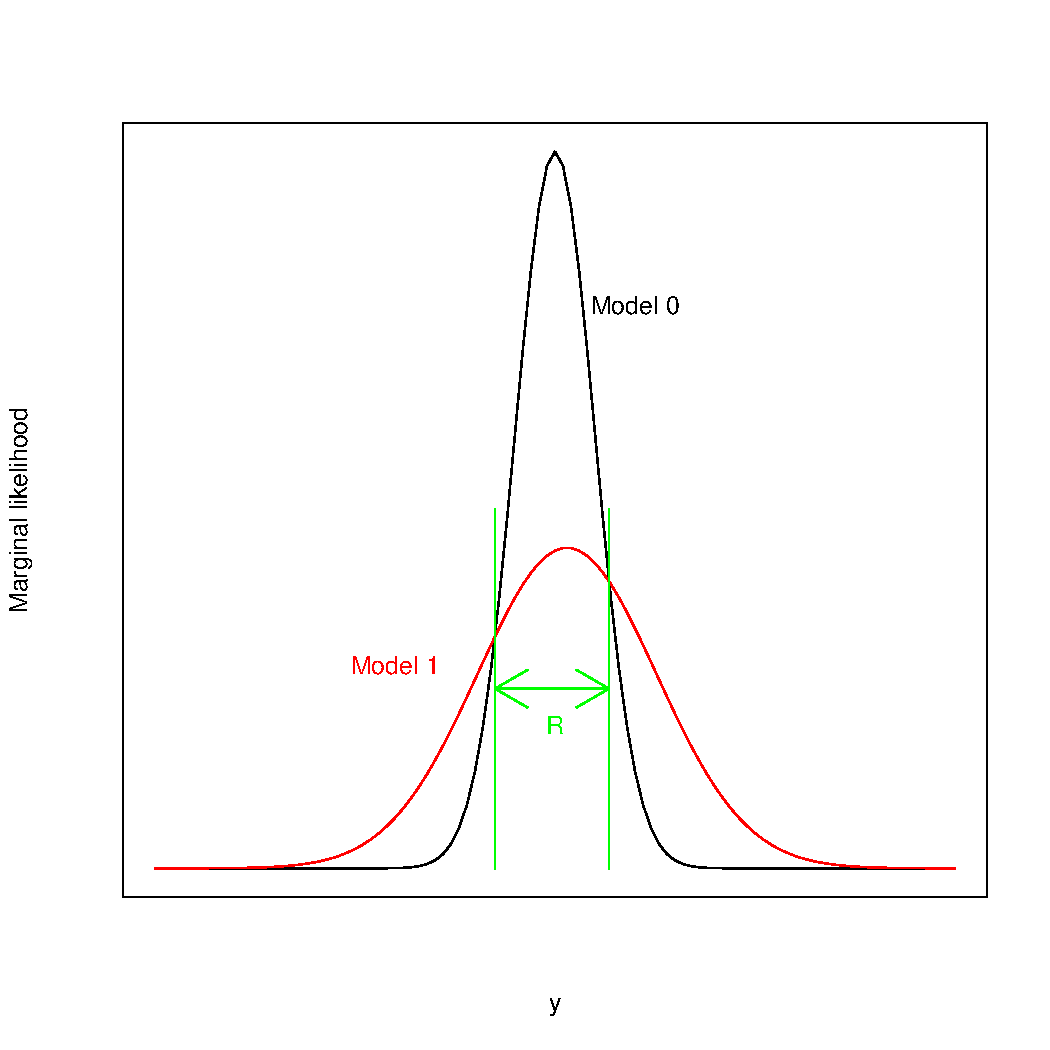
\includegraphics[width=6cm,height=3.5cm]{evidence}}

A simple model, like Model 0, makes only a limited range of predictions; a more powerful model, like Model 1,
that has, for example, more free parameters, is able to predict a greater variety of data sets

\end{slide}

\begin{slide}

\centerline{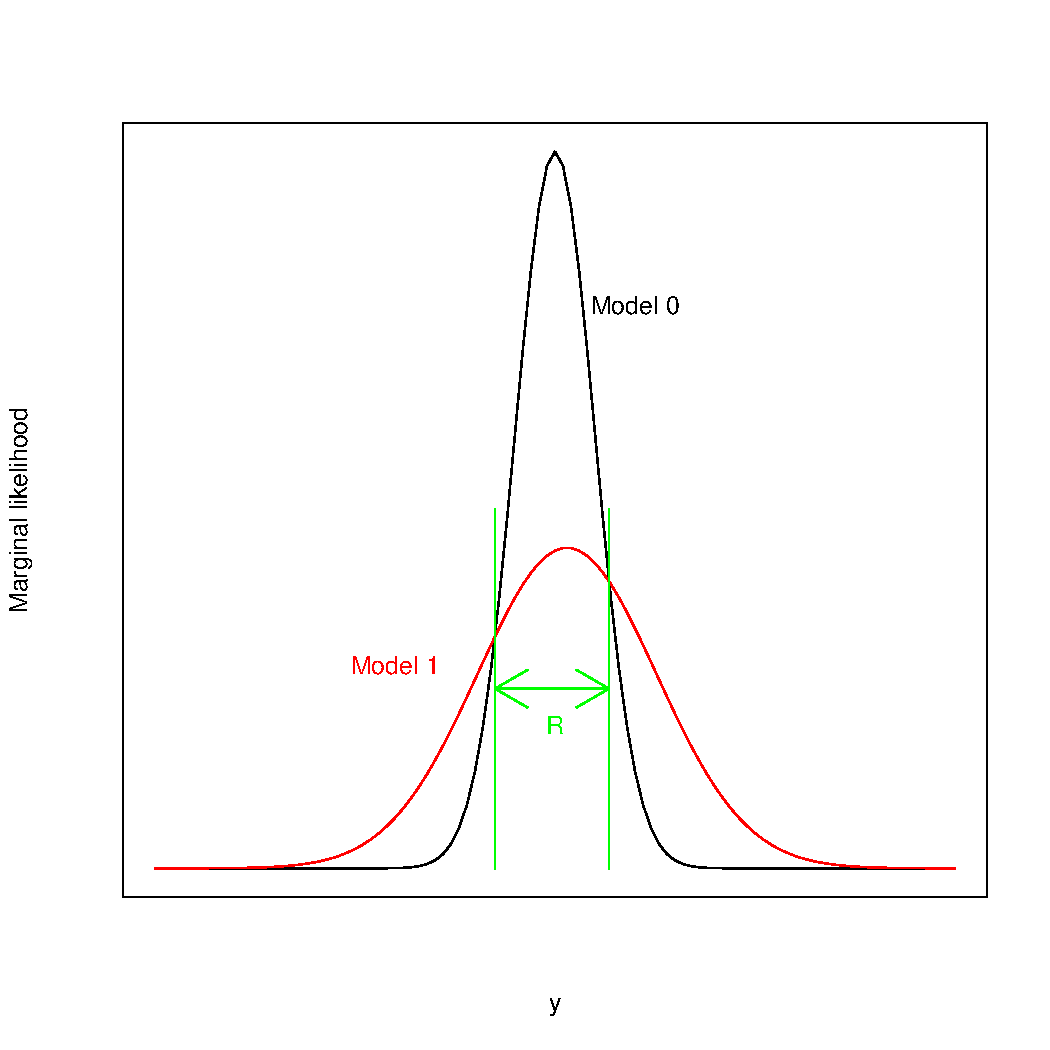
\includegraphics[width=6cm,height=3.5cm]{evidence}}


Suppose that equal prior probabilities have been assigned to the two models. Then, if the data set falls in region R,
the less powerful model will be the more probable model

The marginal likelihood corresponds to a penalized likelihood!

\textbf{\color{red} The BIC information criterium comes from an asymptotic Laplace approximation of the evidence}

\end{slide}

\begin{slide}

\textbf{Bayesian test and model choice: the same problem}

For instance, given a single observation $x|\theta \sim \mathcal{N}(\theta,1)$ 

If $\theta\sim\mathcal{N}(0,1)$, the posterior distribution $\theta|x\sim\mathcal{N}(x/2,1/2)$

If the question of interest is to decide whether $\theta$ is negative or positive, we can directly compute
\begin{eqnarray*}
\P^\pi(\theta<0|x) & = & \P^\pi\left({\sqrt{2}(\theta-x/2)} < {-\sqrt{2}x/2}|x\right) \nonumber\\
                   & = & \Phi\left(-x/\sqrt{2}\right)
\end{eqnarray*}
where $\Phi$ is the standard gaussian cdf

\end{slide}

\begin{slide}

{\bf \color{red} This computation does not seem to follow from the principles we just stated
but it is only a matter of perspective}

Let model 1 be the model such that $\theta<0$ and model 2 the model such that $\theta>0$ 

Using the fact that $\theta\sim\mathcal{N}(0,1)$, we can derive the priors on both models from the original prior 

Let $\pi_1$ be the prior distribution of $\theta$ under model 1, we have
$$
\pi_1(\theta) = 2\dfrac{\exp(-\theta^2/2)}{\sqrt{2\pi}}\,\mathbb{I}_{\theta<0}
$$
a truncated gaussian distribution

\end{slide}

\begin{slide}

Let $\pi_2$ be the prior distribution of $\mu$ under model 2, we have
$$
\pi_2(\theta) = 2\dfrac{\exp(-\theta^2/2)}{\sqrt{2\pi}}\,\mathbb{I}_{\theta>0}
$$
another truncated gaussian distribution

Moreover, using the fact that $\mu\sim\mathcal{N}(0,1)$, we deduce
$$
\P^\pi(\theta<0) = \P^\pi(\theta>0) = 1/2
$$

\end{slide}

\begin{slide}

\begin{equation*}
\begin{split}
 & \int_\mathbb{R} f(x|\theta)\pi_1(\theta)\text{d}\theta= \\
 & \int_{-\infty}^0 \frac{1}{\sqrt{2\pi}} \exp\left(-\frac{1}{2}(x-\theta) ^2\right)\frac{2}{\sqrt{2\pi}}\exp(-\theta^2/2)\text{d}\theta= \\
 & \frac{2\exp(-x^2/4)}{\sqrt{2\pi}\sqrt{2}}\int_{-\infty}^0 \frac{\sqrt{2}}{\sqrt{2\pi}}\exp\left(-(\theta-x/2) ^2\right)\text{d}\theta=\\
 & \frac{2\exp(-x^2/4)}{\sqrt{2\pi}\sqrt{2}}\P^\pi(\theta<0|x)
\end{split}
\end{equation*}

And, with exactly the same type of calculations
\begin{equation*}
\begin{split}
\int_\mathbb{R} f(x|\theta)\pi_2(\theta)\text{d}\theta = \frac{2\exp(-x^2/4)}{\sqrt{2\pi}\sqrt{2}}\P^\pi(\theta>0|x)
\end{split}
\end{equation*}

\end{slide}

\begin{slide}

Then
$$
\P^\pi(\mathfrak{M}=1|x)=\frac{(1/2)\frac{2\exp(-x^2/4)}{\sqrt{2\pi}\sqrt{2}}\P^\pi(\theta<0|x)}{(1/2)\frac{2\exp(-x^2/4)}{\sqrt{2\pi}\sqrt{2}}(\P^\pi(\theta<0|x)+\P^\pi(\theta>0|x))}
$$
$$
\P^\pi(\mathfrak{M}=1|x)=\frac{\P^\pi(\theta<0|x)}{\P^\pi(\theta<0|x)+\P^\pi(\theta>0|x)}
$$
$$
\P^\pi(\mathfrak{M}=1|x)=\P^\pi(\theta<0|x)=\Phi\left(-x/\sqrt{2}\right)=\P^\pi(\theta<0|x)
$$
\textbf{Bayesian test and model choice: the same answer}

\end{slide}

\begin{slide}

\textbf{The Bayes factor}

$$
B^\pi_{21}(\mathcal{D}_n) = \dfrac{ \P^\pi(\mathfrak{M}=2|\mathcal{D}_n) / \P^\pi(\mathfrak{M}=1|\mathcal{D}_n)}
{ \P^\pi(\mathfrak{M}=2)/ \P^\pi(\mathfrak{M}=1)}
$$


While this quantity is a simple one-to-one transform of the posterior probability, it can be used for Bayesian model choice without first resorting to a determination of the prior weights of both models


{\color{red} $$
B^\pi_{21}(\mathcal{D}_n)=\frac{\int_{\Theta_2}\ell_2(\theta_2|\mathcal{D}_n)\pi_2(\theta_2)\,\hbox{d}\theta_2}
{\int_{\Theta_1}\ell_1(\theta_1|\mathcal{D}_n)\pi_1(\theta_1)\,\hbox{d}\theta_1}=\frac{m_2(\mathcal{D}_n)}{m_1(\mathcal{D}_n)}
$$}

\end{slide}


\section{Bayesian Model Averaging}

\begin{slide}

The posterior probabilities in the model space can be used
to average over the decisions coming from different models


Suppose that we are interested in the prediction of
$z$ and that, for model $k$, the predictive distribution of $z$
is $g_k(z|\mathcal{D}_n)$


{\color{red} The average predictive of $z$ is
$$
\sum_{k=1}^J \P^\pi(\mathfrak{M}=k|\mathcal{D}_n)g_k(z|\mathcal{D}_n)
$$}

\end{slide}

\section{Difficulties with the Bayesian model choice paradigm}

\begin{slide}

\vs Prior difficulties: 
\begin{itemize}

\item When we have prior informations, how to choose the prior distributions
on the parameters of each model in a compatible way? 
What about the prior distribution in the models's space? 

\vs \item When we do not have any prior information, \textbf{we can not use improper prior distribution}.
Indeed, in that case, the models's posterior probabilities are only defined up to some arbitrary constants.
How to choose the various prior distributions?
\end{itemize}

\end{slide}

\begin{slide}

Computational difficulties:
\begin{itemize}
\item How to approximate the various posterior probabilities?
\item How to approximate the evidences?
\item When the number of models in consideration is huge, how to explore the models's space?
\end{itemize}

\label{lastslide}

\end{slide}

\end{document}
